\documentclass[10pt, table]{beamer}
\usepackage{graphicx}

\begin{document}
\title{New ACD Calibration Constants' Validation}   
\author{David Green, Terri Brandt, Liz Hays} 
\date{\today} 

\begin{frame}{Plot Needing Approval for AAS Poster}
     \begin{columns}[t] % contents are top vertically aligned
     \begin{column}[T]{0.35 \textwidth} % each column can also be its own environment
      \begin{itemize}
     \item Path length corrected deposited energy vs incident energy
     \item Path length calculated from direction measured by my modified moment analysis
     \item Modified moment analysis has been optimized for hadrons
       \end{itemize}
     \end{column}
     \begin{column}[T]{0.75 \textwidth} % alternative top-align that's better for graphics
          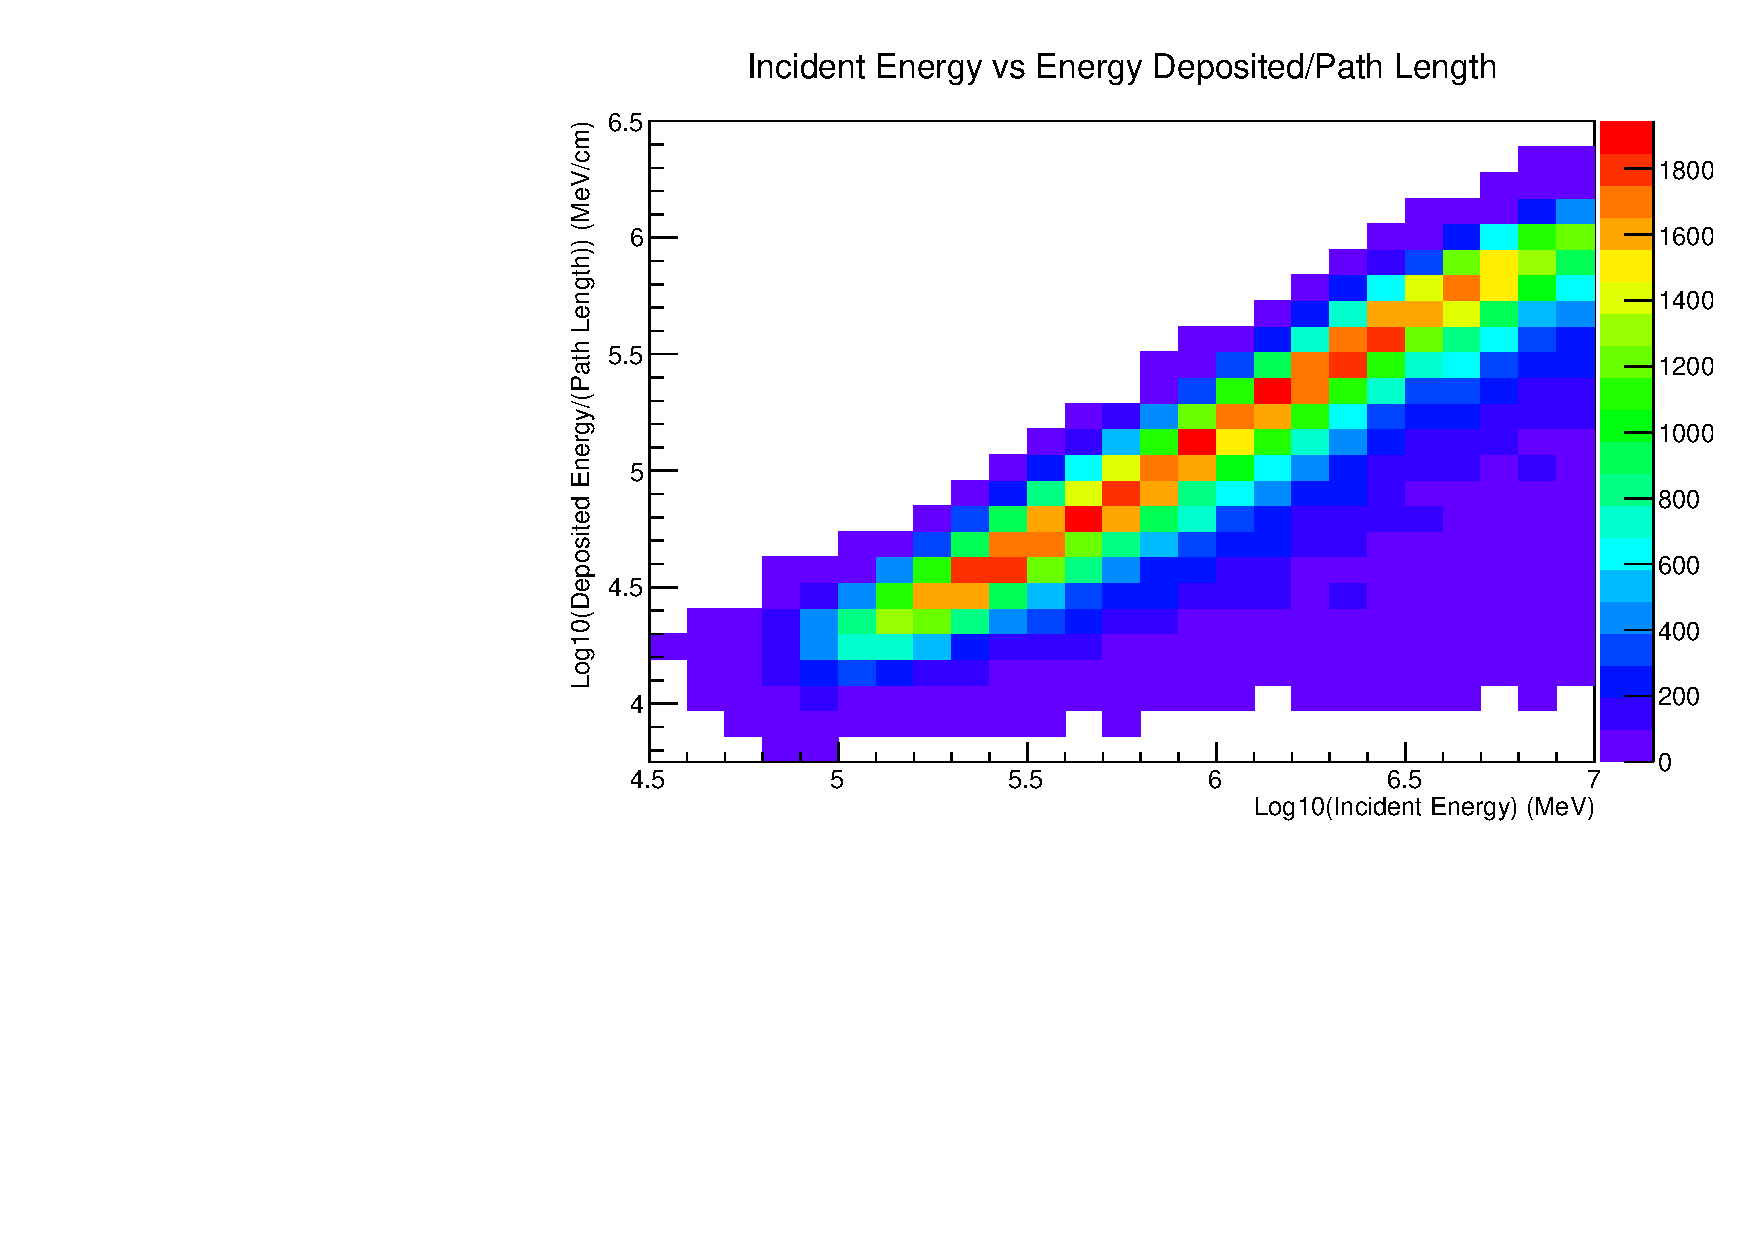
\includegraphics[width = \columnwidth]{CalEnergyRaw-CalFullLen_mom12}
     \end{column}
     \end{columns}
     
    \begin{itemize}
    \item LINK to SB
    \end{itemize}
\end{frame}

%%%

\begin{frame}{Details of the MC}

     \begin{columns}[t] % contents are top vertically aligned
     \begin{column}[T]{0.35 \textwidth} % each column can also be its own environment
      \begin{itemize}
	\item MC produced using v17r35p24gr17
	\item Only boron and carbon nuclei 
	\item Flat energy spectrum from 10 GeV - 10 TeV
	\item Isotropic angular distribution
	\item Require showering events, CalEnergyRaw $\geq$ 20 GeV
	\item Path length $\geq$ 1 nuclear interaction length (380.4 mm)
       \end{itemize}
     \end{column}
     \begin{column}[T]{0.75 \textwidth} % alternative top-align that's better for graphics
          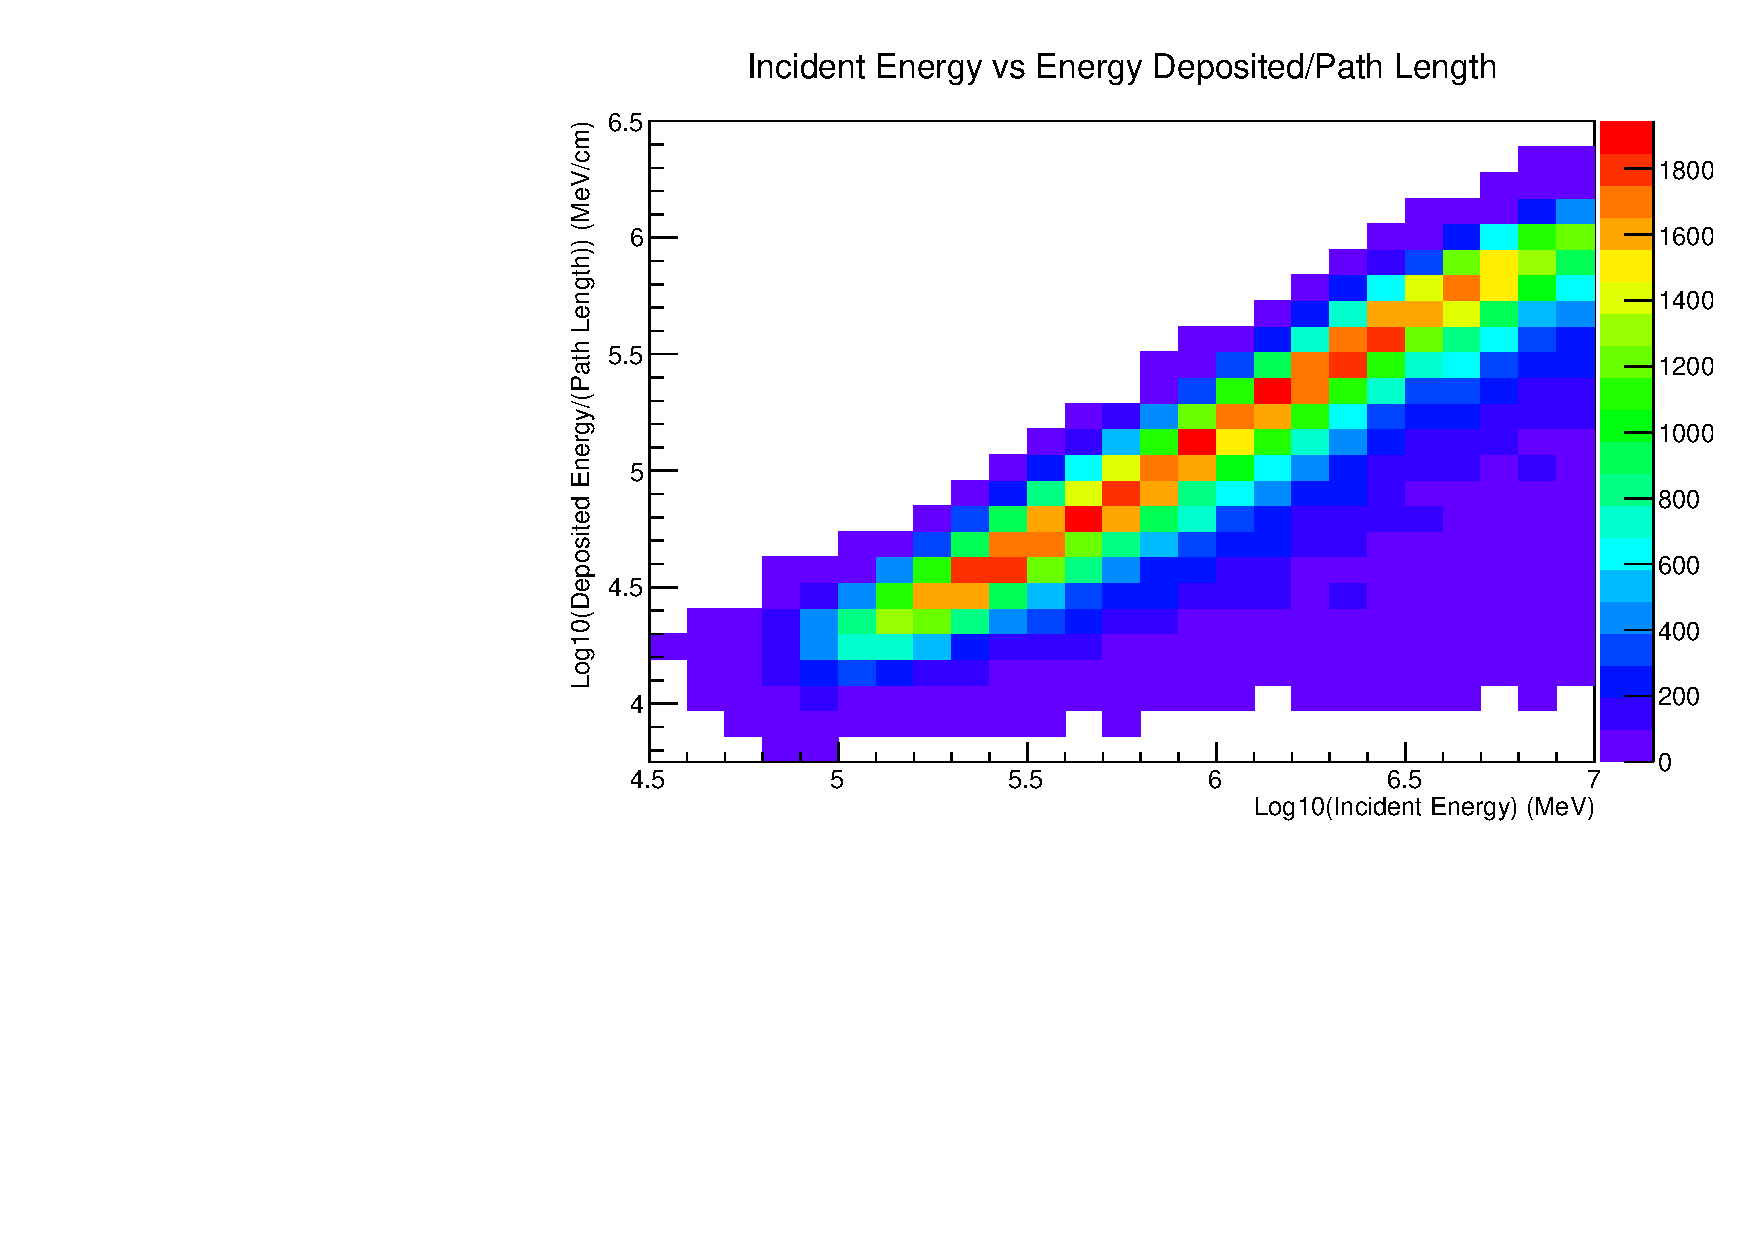
\includegraphics[width = \columnwidth]{CalEnergyRaw-CalFullLen_mom12}
     \end{column}
     \end{columns}

\end{frame}

%%%

\begin{frame}{Modified Moment Analysis}
\begin{columns}[t]
	\begin{column}[T]{0.5 \textwidth}
		\begin{itemize}
			\item We've modified the pass7 moment analysis to improve direction recon for hadrons
			\begin{itemize}
				\item Trim crystals below an energy threshold (400 MeV)
				\item Harder cuts on outlying crystals from core of shower
			\end{itemize}
			\item This results in focusing on the ionization track and electromagnetic core of the hadronic shower, improving direction
			\item Measure containment percentages for $|$CalDir - McDir$|$ in bins of McZDir and McEnergy
		\end{itemize}
	\end{column}
	\begin{column}[T]{0.5 \textwidth}
	          \includegraphics[width = \columnwidth]{psf}
	          
	          \includegraphics[width = \columnwidth]{psf99_2D_pass8_mom}
	\end{column}
\end{columns}	
\end{frame}

%%%

\begin{frame}{Comparing Direction Reconstruction}

	\begin{columns}[t]
	\begin{column}[T]{0.5 \textwidth}
	  \begin{tabular}{|c|c|c|cl} \hline
		          \includegraphics[width = \columnwidth]{psf99_2D_pass8_mom} \\ \hline
		            Modified Moment Analysis \\ \hline
		            \end{tabular}
	\begin{itemize}
	\item Energy and angular dependence on the PSF for various forms of the direction reconstruction
	\item Our modified moment analysis out performs either Pass7  or Pass8
	\end{itemize}
	\end{column}
	\begin{column}[T]{0.5 \textwidth}
		  \begin{tabular}{|c|c|c|cl} \hline
		          \includegraphics[width = 0.9 \columnwidth]{psf99_2D_pass7_old} \\ \hline
		          Pass7 \\ \hline
		          \includegraphics[width = 0.9 \columnwidth]{psf99_2D_pass8_old} \\ \hline
		           Pass8 \\ \hline
		            \end{tabular}
	\end{column}
\end{columns}	
\end{frame}

%%%

\begin{frame}{Comparing Energies}

\begin{center}
  \begin{tabular}{|c|c|c|cl} \hline
           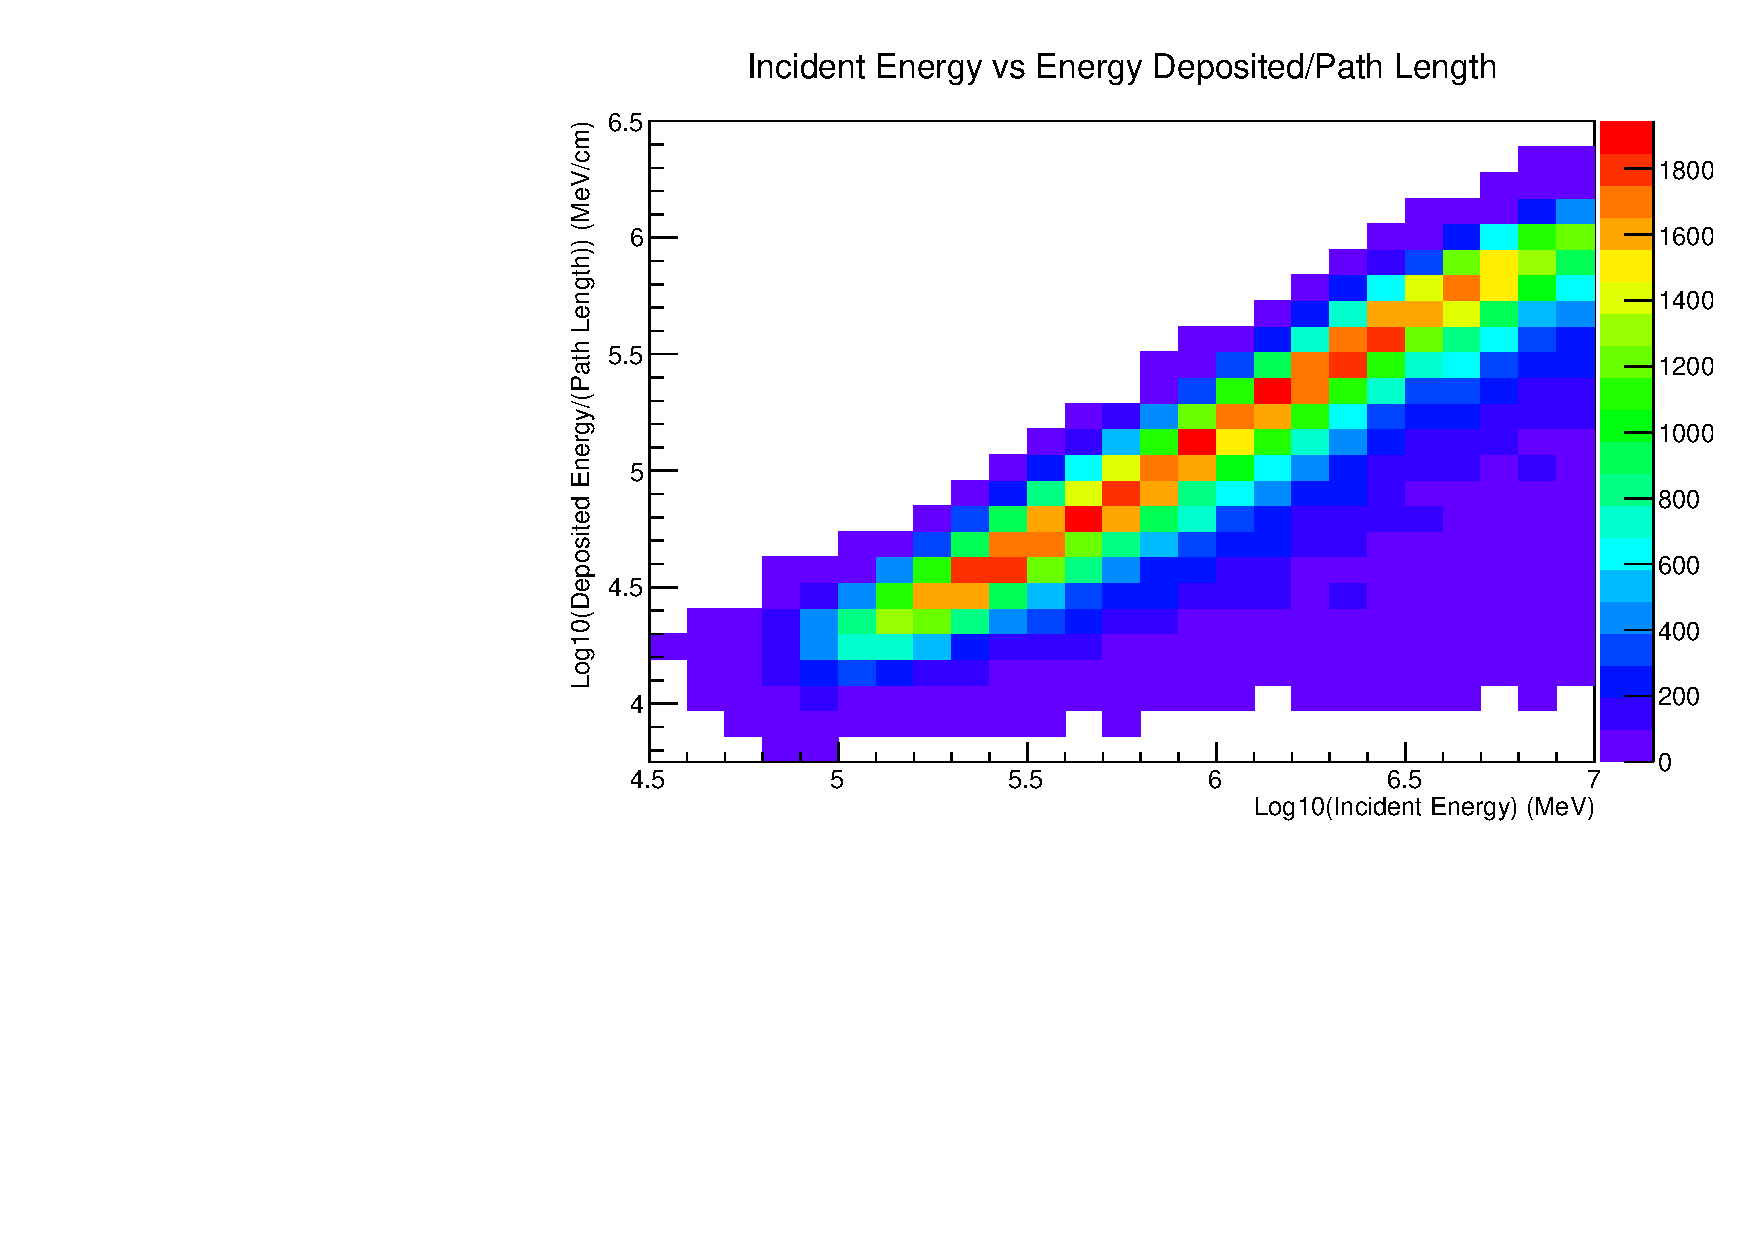
\includegraphics[width = 0.5 \columnwidth]{CalEnergyRaw-CalFullLen_mom12}
 &           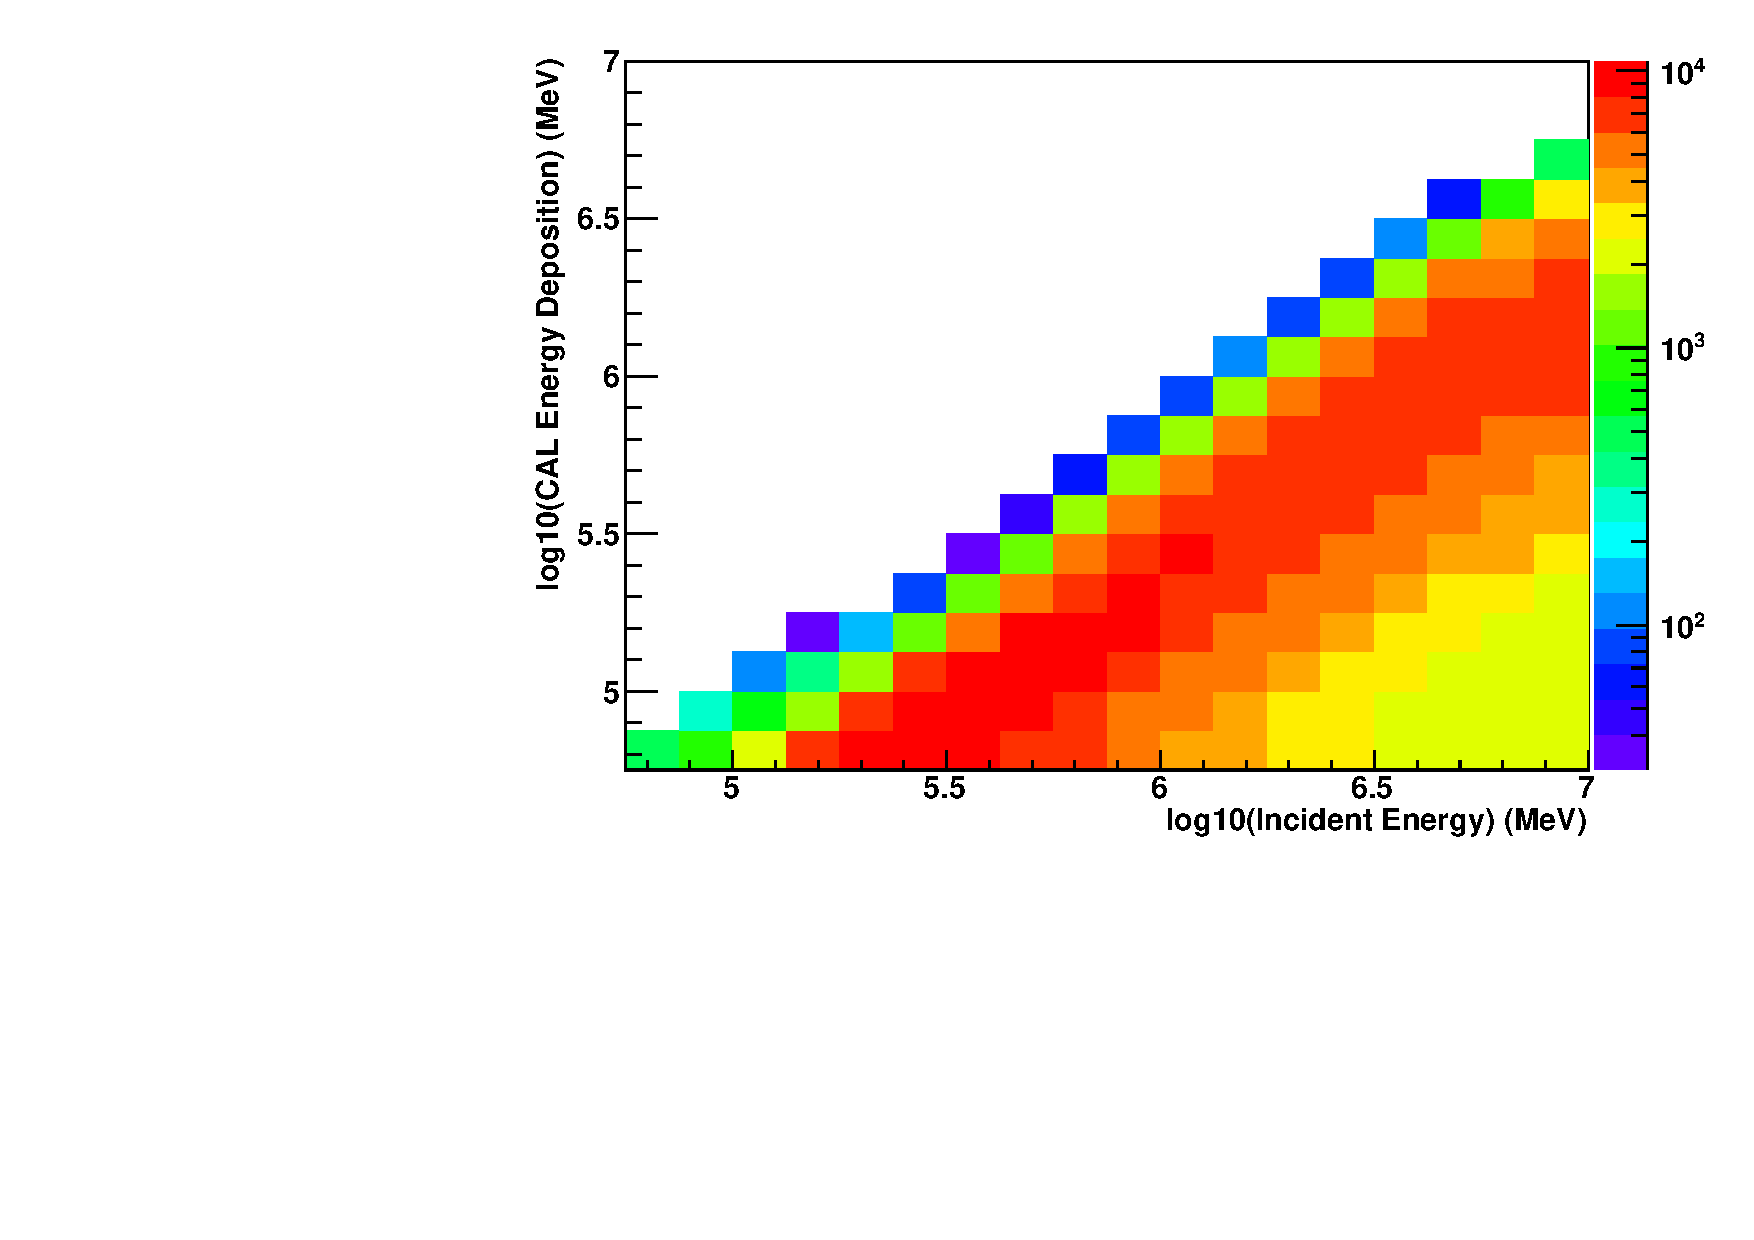
\includegraphics[width = 0.5 \columnwidth]{CalEnergyRaw} \\ \hline
  Modified Energy Comparison & Previous Energy Comparison\\ \hline
  \end{tabular}
  \begin{itemize}
\item We want to show our improved energy analysis for hadrons
\item Demonstrate that measuring hadron energy with LAT is possible
\item Modified energy resolution on the order of 30\% (Comparable to other thin calorimeters)
\end{itemize}
\end{center}

\end{frame}

%%%

\end{document}

